\documentclass[11pt,oneside,a4paper]{article}
\usepackage[%
  a4paper,%
  left = 20mm,%
  right = 20mm,%
  textwidth = 160mm,%
  top = 40mm,%
  bottom = 30mm,%
  %heightrounded,%
  headheight=70pt,%
  headsep=25pt,%
]{geometry}
\usepackage{graphicx}
\usepackage{listings}
\usepackage{tikz}

% Added Packages
\usepackage[defaultfam,tabular,lining]{montserrat}
\usepackage{seqsplit}
\usepackage[pages=some]{background}

\usepackage{hyperref}
\hypersetup{
    colorlinks = true,
    allcolors  = black, 
}
\usepackage{nameref}
\usepackage{lastpage}
\usepackage{graphicx}
\usepackage{float}
\usepackage{xspace}
\usepackage{longtable}
\usepackage{tabularx}
\usepackage{color,colortbl}

\definecolor{link-blue}{RGB}{6,69,173}
\definecolor{dark-green}{RGB}{52,133,62}
\definecolor{light-blue}{RGB}{127,180,240}
\definecolor{dark-blue}{RGB}{72,120,224}
\definecolor{heading-grey}{RGB}{128,128,128}
\definecolor{heading2-grey}{RGB}{200,200,200}
\definecolor{dark-al}{RGB}{22,22,22}
\definecolor{white-al}{RGB}{242,242,242}
\definecolor{Critical}{RGB}{192,0,0}
\definecolor{Major}{RGB}{255,0,0}
\definecolor{Medium}{RGB}{255,192,0}
\definecolor{Minor}{RGB}{255,255,0}
\definecolor{Informational}{RGB}{94,185,255}

% Define colors
\definecolor{codegreen}{rgb}{0,0.6,0}
\definecolor{codegray}{rgb}{0.5,0.5,0.5}
\definecolor{codepurple}{rgb}{0.58,0,0.82}
\definecolor{backcolour}{rgb}{0.95,0.95,0.92}

% Code listing style
\lstdefinestyle{mystyle}{
    backgroundcolor=\color{backcolour},   
    commentstyle=\color{codegreen},
    numberstyle=\tiny\color{codegray},
    stringstyle=\color{codepurple},
    basicstyle=\ttfamily\footnotesize,
    breakatwhitespace=false,         
    breaklines=true,                 
    captionpos=b,                    
    keepspaces=true,                 
    numbers=left,                    
    numbersep=5pt,                  
    showspaces=false,                
    showstringspaces=false,
    showtabs=false,                  
    tabsize=2,
    morekeywords={data, type, deriving, class, instance, Maybe, Integer, Generic}
}

\lstset{style=mystyle}

\usepackage{listings}
\usepackage{enumitem}
\usepackage{array,booktabs}
\usepackage{fancyhdr}
\renewcommand{\footrulewidth}{0.2pt}
\renewcommand{\headrulewidth}{0.2pt}
\fancyfoot{}
\fancyhead{}
\fancyfoot[C]{Confidential}

\usepackage[skip=10pt plus1pt, indent=0pt]{parskip}

\usepackage[T1]{fontenc}
\renewcommand*\oldstylenums[1]{{\firaoldstyle #1}}

\newcommand\projectno{Money Kit }


\backgroundsetup{
  scale=1,
  opacity=0.9,
  angle=0,
  contents={
\includegraphics[width=\paperwidth,height=\paperheight]{img/background-1.jpg}}
}

\begin{document}

\renewcommand{\headrulewidth}{0pt}

% \pagenumbering{gobble}

%%%%%%%%%%%%%%%%%%%%%%%%%%%%%%%%%%%%%%%%%
%%          Begin title page           %%
%%%%%%%%%%%%%%%%%%%%%%%%%%%%%%%%%%%%%%%%%
\pagecolor{dark-al}
\BgThispage
\clearpage

\begin{titlepage}
    \begin{center}
        \vspace*{8em}

        \centering
\includegraphics[width=10cm]{img/Logo-Anastasia-Labs-V-Color02.png}

        \vspace{3em}

        \huge{\textcolor{white-al}{\textbf{Trustless P2P On-Ramp Smart Contract Design Specification}}}

        \vspace{10em}

    \end{center}

    \textcolor{white-al}{Date: \today} \\
    \textcolor{white-al}{Project: \projectno} \\
    \textcolor{white-al}{Version 1.0}

\end{titlepage}

\renewcommand{\headrulewidth}{0.2pt}

\pagecolor{white}
\newpage

\fancypagestyle{plain}{
    \fancyfoot[C]{\textcolor{heading-grey}{\textbf{Anastasia Labs -- \projectno} \\ Confidential \\ Copyright ©  \href{https://anastasialabs.com/}{Anastasia Labs}}}
    \fancyhead[R]{
\includegraphics[width=4cm]{img/Logo-Anastasia-Labs-V-Color01.png}}
}
\pagestyle{plain}

\newpage

\fancypagestyle{plain}{
    \fancyfoot[R]{\\ \textcolor{heading-grey}{\newline Page \thepage\ of \pageref{LastPage}}}
    \fancyfoot[C]{\textcolor{heading-grey}{\textbf{Anastasia Labs -- \projectno} \\ Confidential \\ Copyright ©  \href{https://anastasialabs.com/}{Anastasia Labs}}}
    \fancyhead[R]{
\includegraphics[width=4cm]{img/Logo-Anastasia-Labs-V-Color01.png}}
}

\pagestyle{plain}
% \pagenumbering{arabic}

%%%%%%%%%%%%%%%%%%%%%%%%%%%%%%%%%%%%%%%%
%           Begin contents            %%
%%%%%%%%%%%%%%%%%%%%%%%%%%%%%%%%%%%%%%%%

\section{Introduction}
This document provides a detailed technical protocol design specification for a Trustless P2P On-Ramp smart contract application. The system is designed to connect cryptocurrency sellers and buyers in a decentralized manner, ensuring the secure transfer of funds with minimal trust required between parties. The application leverages Money Kit for user registration and transaction validation.

\section{Key Components}
\begin{enumerate}
    \item \textbf{Money Kit Integration} Ensures that both buyers and sellers are registered and validated
    \item \textbf{Smart Contract} Manages fund deposits, timelocks, and the release of the funds based on cryptographic proof
    \item \textbf{Cryptographic Proof} Mechanism for the buyer to prove fiat payment delivery
    \item \textbf{Timelocked Transactions} Ensures funds are held securely until conditions are met
    \item \textbf{Non-Compliance Mechanism} Handles cases where buyers do not follow through with the purchase
\end{enumerate}

\section{Protocol Design}

\subsection{Data Structures}

\begin{lstlisting}[language=Haskell]
data Datum = Datum
  { paymentInfoHash :: ByteString
      -- ^ Hashed payment information
  , sellPriceUsd :: Integer
      -- ^ Price in USD for the sale
  , valueSold :: Value
      -- ^ Cryptocurrency value being sold
  }
\end{lstlisting}

\subsection{Registration}
Buyer and Seller Registration
\begin{itemize}
    \item Both parties must register via MoneyKit.

\end{itemize}

\subsection{Transaction Phases}

\subsubsection{Intent to Buy}

\begin{itemize}
    \item Buyer submits an intent to buy.
    \item Fiat account information (hashed) is shared with the seller.
    \item Transaction is created and timelocked with the seller's funds in the UTxO.
\end{itemize}

\subsubsection{Timelock Phase}

\begin{itemize}
    \item Transition to the timelock phase requires a signed message from MoneyKit, validating the buyer's registration.
    \item MoneyKit provides a signed message validating the user's registration and Cardano address.
    \item Only validated orders are shown in the UI.
\end{itemize}

\subsubsection{Payment and Fund Release}

\begin{itemize}
    \item Funds are timelocked for a specified period (e.g., 15 blocks after payment is made).
    \item The buyer generates a cryptographic proof of payment and submits it to the smart contract.
    \item Upon successful verification, the funds are released to the buyer.
\end{itemize}

\subsubsection{Non-Compliance Handling}

\begin{itemize}
    \item If the buyer submits an intent to buy and does not follow through, the associated MoneyKit account is banned.
\end{itemize}

\begin{figure}[h]
\centering
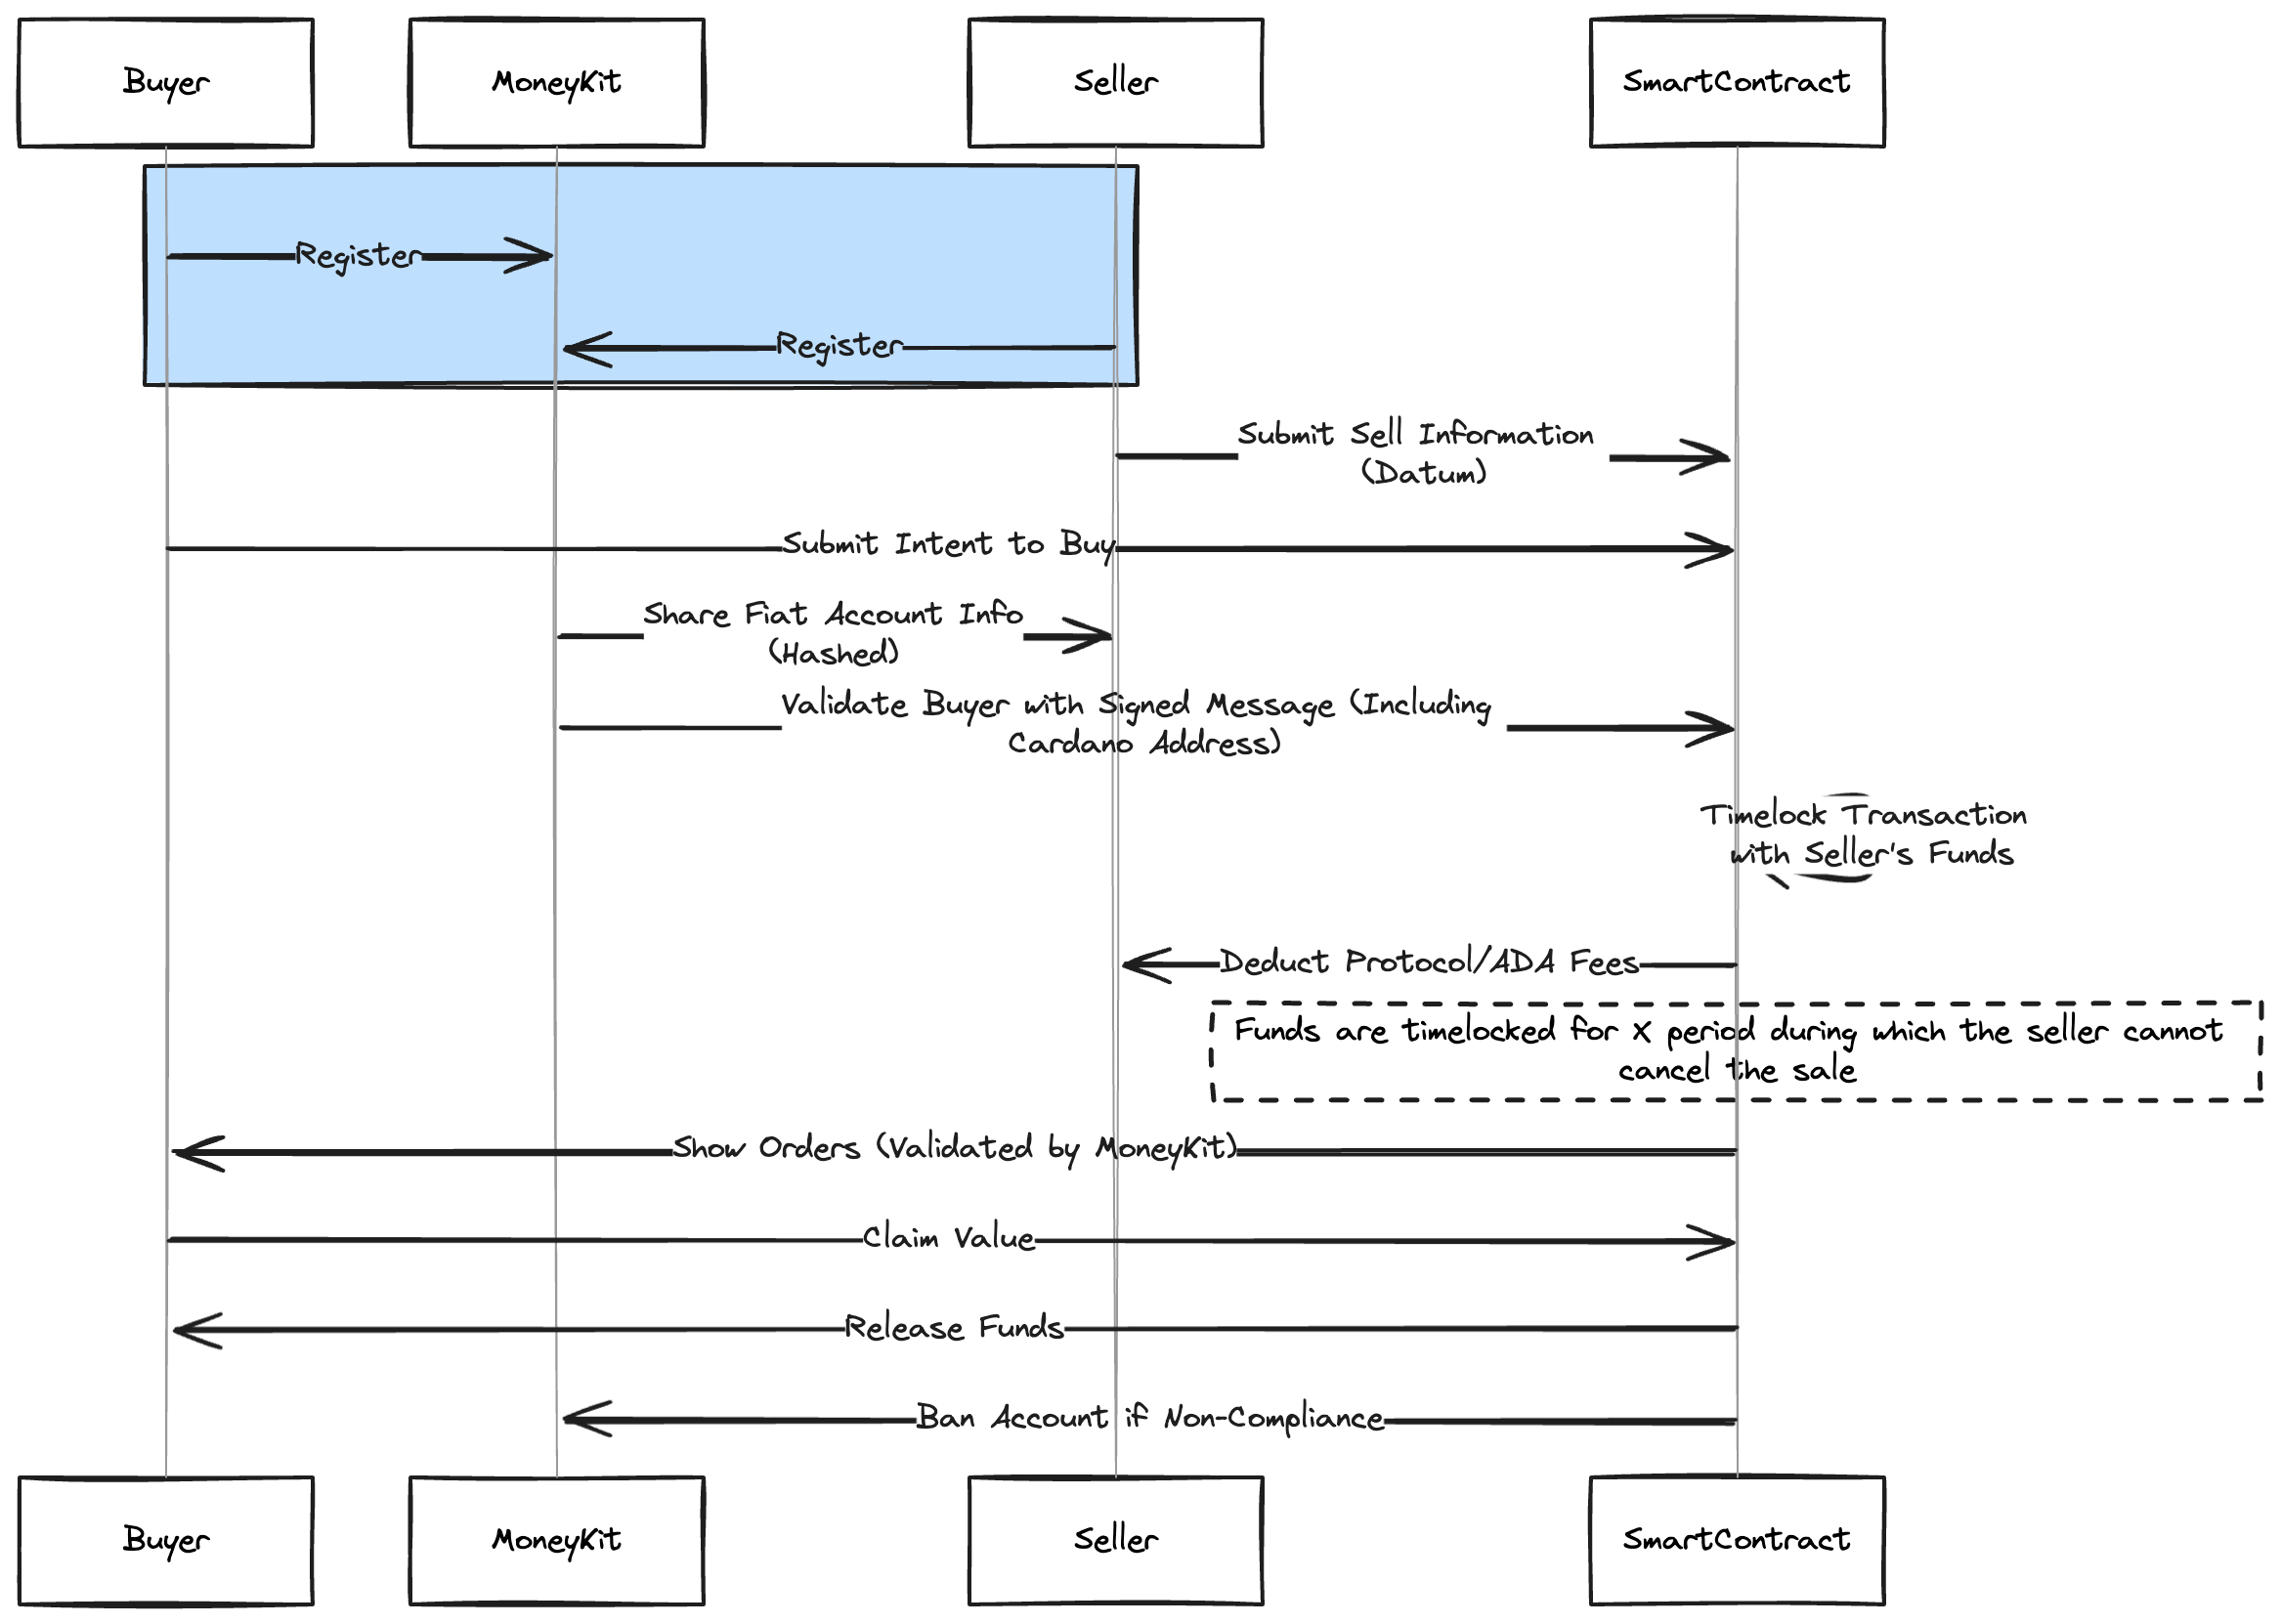
\includegraphics[width=0.8\textwidth]{img/money_kit.png}
\end{figure}

\section{Security Considerations}

\begin{itemize}
    \item \textbf{Timelock}:
    \begin{itemize}
        \item Ensure timelock duration is sufficient for payment confirmation.
        \item Protect against replay attacks using unique transaction IDs.
    \end{itemize}

    \item \textbf{Cryptographic Proof}:
    \begin{itemize}
        \item Use robust cryptographic methods to ensure proof cannot be forged.
    \end{itemize}

    \item \textbf{Non-Compliance}:
    \begin{itemize}
        \item Implement a reliable mechanism to detect and handle non-compliance by buyers.
    \end{itemize}
\end{itemize}

\section{Conclusion}

This specification outlines the design and implementation of a Trustless P2P On-Ramp smart contract application. By leveraging MoneyKit for user validation and implementing secure smart contract logic, the system ensures a trustless and secure environment for cryptocurrency transactions.


\end{document}
